\documentclass[11p, titlepage]{article}

\usepackage[a4paper, portrait, margin=0.9in]{geometry}
\setlength{\parskip}{1em}

\usepackage[hidelinks]{hyperref}

\usepackage{graphicx}
\graphicspath{ {./images/} }
\usepackage{caption}
\usepackage{subcaption}
\captionsetup[subfigure]{justification=centering}
\usepackage{wrapfig}

\title{COSC470 Research Project Report\\
\bigskip
Contour Splitting for Branching Structures in CT Image Reconstructions}
\author{Cameron Stevenson\\[0.5cm]{\small Supervisor: Ramakrishnan Mukundan}}

\begin{document}

\maketitle
\abstract{abstract text}
\tableofcontents

\section{Overview}

overview text
Example citation \cite{mackay2019robust, mukundan2016reconstruction, pan2017comparison}.
Example URL \footnote{\url{https://github.com/cstevenson3/cosc470writing/blob/main/survey.pdf}}.

\section{Introduction}

introduction text

\section{Background}

We begin with a look at typical methods in rendering scan data. Then, correspondence methods are looked at in depth as the approach this report builds upon.

\subsection{Overview}

Images from scans (also referred to as sections or slices) can be segmented based on intensity into pixel regions to define structure boundaries. These can be processed further by finding contours to represent these boundaries.

Any medical imaging reconstruction/render is typically concerned with a particular area of the body, dependent on the application. Most applications tend to use either volumetric rendering or surface rendering.

Volumetric rendering treats pixels in images as voxels, and a variety of rasterization and raycasting techniques are available for rendering these.

Surface rendering requires a surface be defined, either implicitly or as a mesh. Point cloud methods generate implicit surfaces, whilst meshes can be generated through contour correspondence followed by mesh triangulation (with point correspondence as an optional middle step). 

\subsection{Applications}

Xuyi et al. \cite{xuyi2016application} use 3D reconstructions from hip CT scans to make patient-specific surgery plans. From the model they measure the direction and degree of the acetabular fragment, and use this to guide their surgery.

Pan et al. \cite{pan2017comparison} refers to the importance of 3D reconstructions and rendering in robot-assisted surgery. With real time rendering being a priority, surface reconstructions are preferred over volume rendering. Of the four methods analysed, marching cubes was found to be the most suitable due to its speed and render quality.

Lim et al \cite{lim2016use} found that the use of 3D printed cardiac models in education resulted in a statistically significant improvement in test scores of medical students.

\subsection{Scanning and Image Processing}

As with most areas involving measurement of the real world, unwanted artefacts such as noise are introduced in the imaging process. There can also be variation from subject to subject and between imaging machines. Therefore standard image processing techniques are used to pick out the parts of images which are relevant to the application. Running signal processing on the 2D data (as opposed to considering the whole image stack in the reconstruction stage) reduces complexity. However techniques considering the image data from all slices have been considered.

\subsubsection{Segmentation}

Segmentation is the process of picking out the pixels belonging to individual objects in an image. From this the projected geometry of the object onto the image can be inferred, which is then used in reconstruction or rendering. Birkfellner \cite{birkfellner2016applied} observes that organs are usually composed of multiple tissue types, which show up as different intensities under imaging. This makes segmentation "a rather complex, specialized procedure often requiring considerable manual interaction". Particular organs are often focussed on when developing segmentation methods.

Birkfellner \cite{birkfellner2016applied} covers some advanced segmentation methods. The watershed transform for example uses the physical idea of water running to the bottom of valleys in a landscape. After taking a gradient transform on an image, edges are peaks in the landscape, and the virtual water will fill up basins representing segments in the image. Various interpretations of the physical behaviour can be used.

Carr \cite{carr1996surface} refers to various morphological methods used to remove noise. An opening operation acts like a low pass filter whilst still preserving edges. Opening and closing in sequence tends to be better at maintaining the mean intensity.

Mukundan \cite{mukundan2016reconstruction} observes that in HRCT lung scans, tissue regions are "characterized by different and easily separable intensity levels". In this case simple thresholding can be used to pick out regions. 

\subsubsection{Contour Finding}

Rather than use pixels/voxels, some reconstruction techniques use contours defining the boundaries of the region objects occupy in an image. 

Mukundan \cite{mukundan2016reconstruction} starts with a binary image after thresholding. Eroding the image with a 3x3 element then subtracting this from the thresholded image gives one pixel wide edges. Sequential edge following is used to extract contours. Discarding small contours reduces the number of contours significantly.

Pu et al. \cite{pu2008adaptive} introduce a border marching algorithm with an adaptive step size to find the outer contours of the lungs. The metric for adjusting the step size for a border segment is based on how far (at most) the segment lies from the true border. This method has the advantage of including small juxtapleural pulmonary modules in the segmentation despite their imaged intensity being dissimilar to the rest of the lung. Mackay \cite{mackay2019robust} uses this method.

\subsubsection{Contour Interpolation}

Between two slices filled with contours, new slices can be added with contours interpolated from those in the slices above and below them. Some methods are able to do this without a contour correspondence.

Barrett et al. \cite{barrett1994image} present a contour interpolation algorithm in image space based on morphological operations. An image with both contours present (as different grayscale values) is dilated until the space between contours is filled. The front where the two dilations meet is where the interpolated contour is found. It is noted that this method handles branching cases with no modification necessary.

Chai et al. \cite{chai1998contour} use partial differential equations to interpolate between contours on a terrain map. Their method produces smooth interpolations, and can handle complex shapes such as two or three branches.

\subsection{Typical Methods}

generic methods text

\subsection{Correspondence Methods}

subsection preamble text

\subsubsection{Contour Correspondence}

contour correspondence text

Example list:
\begin{itemize}
\item item1
\item item2
\item item3
\end{itemize}

\subsubsection{Point Correspondence and Triangulation}

pc and t text

\begin{figure}[h]
     \centering
     \begin{subfigure}[b]{0.2\textwidth}
         \centering
         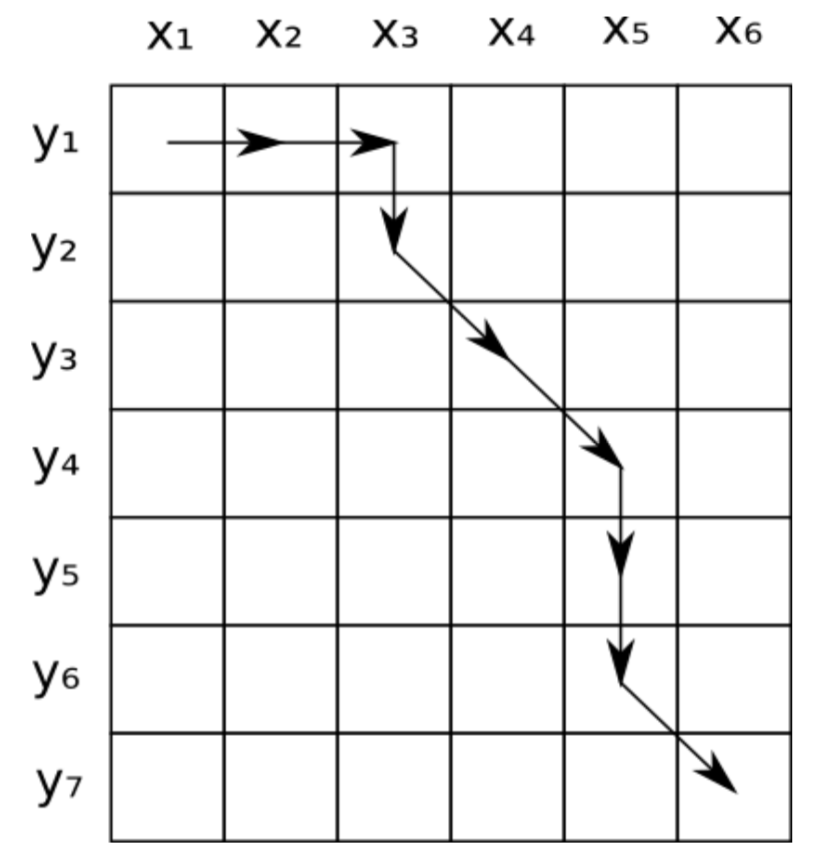
\includegraphics[width=\textwidth]{dtw1}
         \caption{DTW path through cost matrix}
         \label{fig:dtw1}
     \end{subfigure}
     \hfill
     \begin{subfigure}[b]{0.6\textwidth}
         \centering
         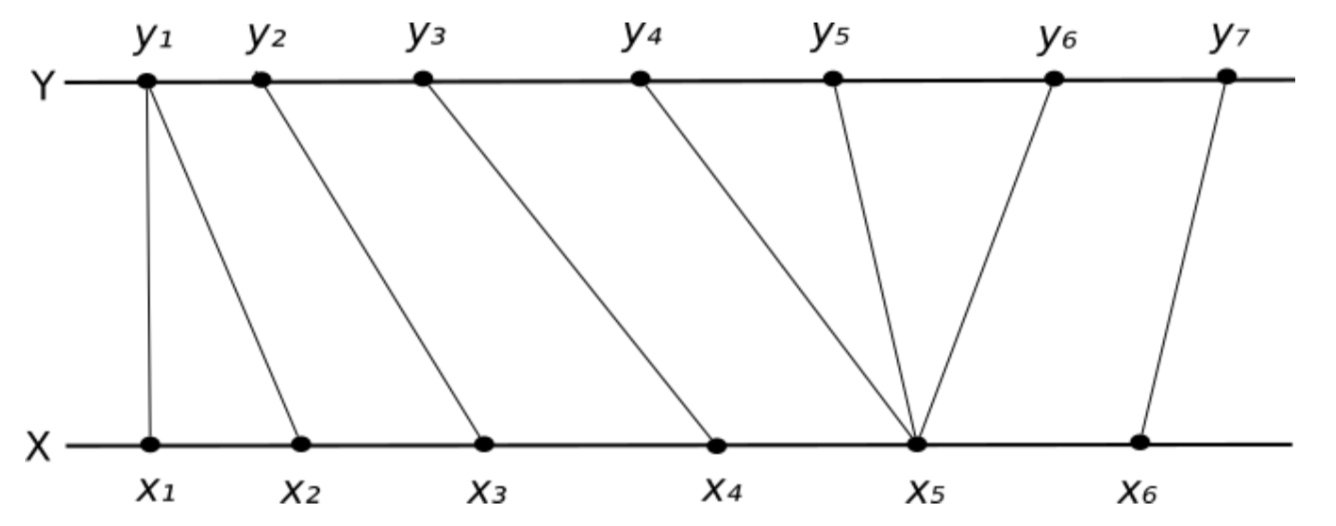
\includegraphics[width=\textwidth]{dtw2}
         \caption{DTW point correspondence}
         \label{fig:dtw2}
     \end{subfigure}
        \caption{Two examples of DTW paths on contours X and Y \cite{mackay2019robust}}
        \label{fig:dtw}
\end{figure}

text after figure declaration

\subsubsection{Branching Problem}

branching problem text

\section{Method}

method text

\subsection{Proposal}

\begin{wrapfigure}{r}{0.25\textwidth}
\centering
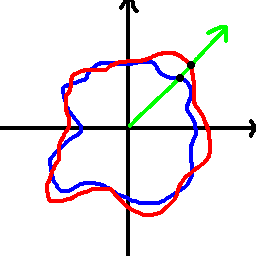
\includegraphics[width=0.2\textwidth]{pa}
\caption{Points matched by angle from shared centroid\label{fig:pa}}
\end{wrapfigure}

The proposed system consists of:
\begin{itemize}
\item Contour Splitting, a new approach to enabling point correspondence on branches and other structures
\item Point Angle, an alternative algorithm for point correspondence.
\end{itemize}

Example figure ref (See Figure \ref{fig:pa}).

\subsubsection{Contour Splitting}

For brevity, contour correspondences of 1-to-2 will be considered. Point correspondence algorithms act on 1-to-1 contour matchings, so 1-to-2 cases must be reduced to these. 

Mackay's approach was contour merging, where the 2 contour side of the correspondence is merged. The closest pair of points across the contours is found, to join them into a single contour (See Figure TODO). This gives a single 1-to-1 case for point correspondence to act on. A disadvantage of this method is that the merged contour has an unusual shape, which can cause point correspondence algorithms to behave poorly.

The proposed technique instead splits the 1 contour side of the correspondence. The best fit line to divide the 2 contour side is found, giving the angle of the line to split the 1 contour (See Figure TODO). Each half of the split 1 contour is paired with its corresponding contour on the 2 contour side. This gives two 1-to-1 cases for point correspondence to act on. The contours produced are well shaped and suitable for point correspondence algorithms designed for simpler cases.

Adjustments can be made to the position of the split line to improve accuracy. 
\begin{itemize}
\item The ratio of contour areas on the 2 contour side can be reflected in the split contour by adjusting which points the split line connects to. This preserves the internal cross section of each branch half as they join. 
\item To achieve a smooth point correspondence along the inside of the branch (where the branches join each other), the split line must have points added along it. This is in proportion to the number of points on the original contour.
\item The split line may also be adjusted in height, to reflect the likelihood the branch split is somewhere between the two planes of contours. With no further calculation, the height is assumed to be halfway. A semi-circular curve creates a split line joint which mimics the intersection of two cylinders, which is approximately what is expected from two branches coming together.
\end{itemize}

\subsubsection{Point Angle}

Prior methods of point correspondence consider the Euclidean distance between points on corresponded contours. The proposed algorithm instead considers similar angular distance relative to the contour's centroid. For contours where every border point can be seen from the centroid (similar to star-shaped polygons), the angular distance metric is monotonically increasing. In point correspondence, the contours' point angle metrics are leapfrogged between to join points (See Figure TODO). This leapfrogging assumes the monotonically increasing property. For contours which "double back" (are not star-shaped), the monotonically increasing property can be enforced when filling in the point angle metric, by recording the previous angle if the current angle is smaller. This can lead to sections of points with the same point angle metric, and leapfrogging which produces unideal many-to-one mappings. To counter this, a second metric is added, which is simply progression along the number of points in the contour, starting from the same point as the angle metric. These two metrics are weighted and summed before the leapfrogging correspondence.

\subsection{Implementation}

Mackay's report provides a complete implementation of contour and point correspondence (TODO cite software). This implementation was modified to add the options of contour splitting and point angle for point correspondence. The modified source code is available here (TODO git link).

\begin{figure}[h]
     \centering
     \begin{subfigure}[b]{0.22\textwidth}
         \centering
         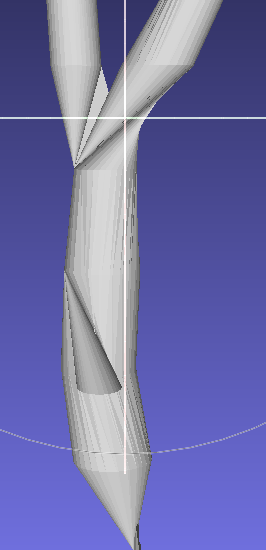
\includegraphics[width=\textwidth]{dtw10}
         \caption{DTW \linebreak}
         \label{fig:dtw10}
     \end{subfigure}
     \hfill
     \begin{subfigure}[b]{0.2\textwidth}
         \centering
         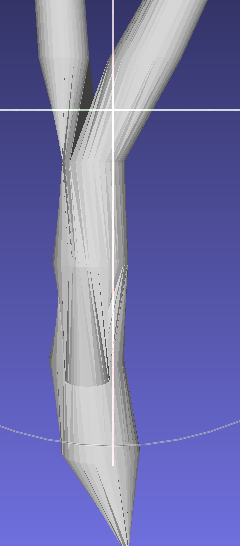
\includegraphics[width=\textwidth]{pa10ang00}
         \caption{Point angle, 0\% angle weight}
         \label{fig:pa10ang00}
     \end{subfigure}
     \hfill
     \begin{subfigure}[b]{0.195\textwidth}
         \centering
         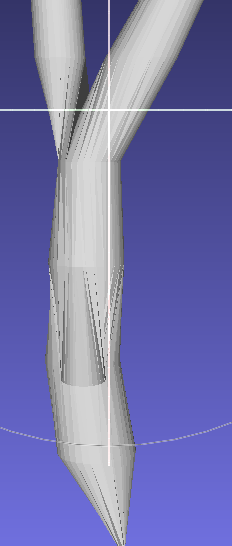
\includegraphics[width=\textwidth]{pa10ang50}
         \caption{Point angle, 50\% angle weight}
         \label{fig:pa10ang50}
     \end{subfigure}
     \hfill
     \begin{subfigure}[b]{0.2\textwidth}
         \centering
         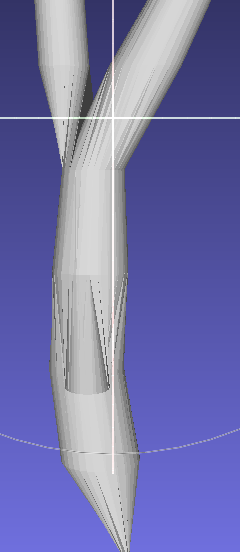
\includegraphics[width=\textwidth]{pa10ang100}
         \caption{Point angle, 100\% angle weight}
         \label{fig:pa10ang100}
     \end{subfigure}
        \caption{Reconstructions with 10 plane samples}
        \label{fig:plane10}
\end{figure}

\begin{figure}[h]
     \centering
     \begin{subfigure}[b]{0.215\textwidth}
         \centering
         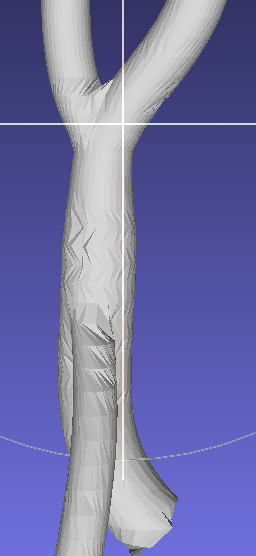
\includegraphics[width=\textwidth]{dtw50}
         \caption{DTW \linebreak}
         \label{fig:dtw50}
     \end{subfigure}
     \hfill
     \begin{subfigure}[b]{0.2\textwidth}
         \centering
         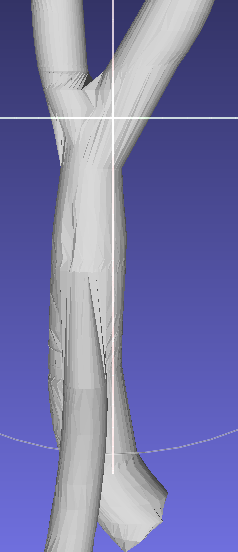
\includegraphics[width=\textwidth]{pa50ang00}
         \caption{Point angle, 0\% angle weight}
         \label{fig:pa50ang00}
     \end{subfigure}
     \hfill
     \begin{subfigure}[b]{0.205\textwidth}
         \centering
         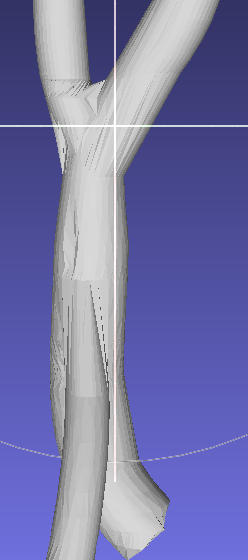
\includegraphics[width=\textwidth]{pa50ang50}
         \caption{Point angle, 50\% angle weight}
         \label{fig:pa50ang50}
     \end{subfigure}
     \hfill
     \begin{subfigure}[b]{0.2\textwidth}
         \centering
         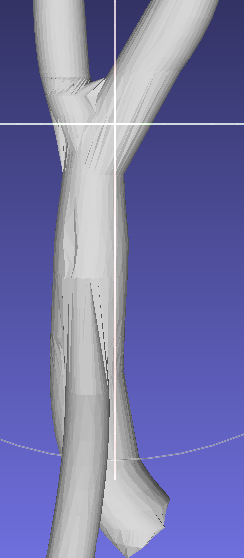
\includegraphics[width=\textwidth]{pa50ang90}
         \caption{Point angle, 90\% angle weight}
         \label{fig:pa50ang90}
     \end{subfigure}
        \caption{Reconstructions with 50 plane samples}
        \label{fig:plane50}
\end{figure}

\section{Analysis}

analysis text

\subsection{Ground Truth}

ground truth text

\subsection{Visual Results}

visual results text

\subsection{Measurements}

measurements text

\subsection{Summary}

summary text

\section{Conclusion}

conclusion text

\pagebreak
\bibliographystyle{IEEEtran}
\bibliography{references}

\section{Appendix}

\begin{figure}[h]
\centering
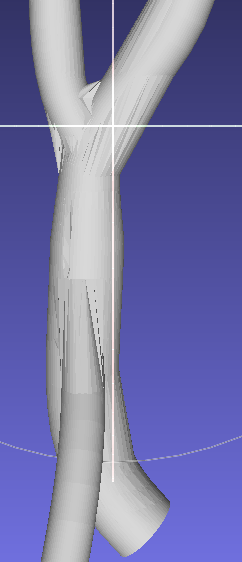
\includegraphics[width=0.29\textwidth]{mb}
\caption{Original multi branch model\label{fig:model}}
\end{figure}

\end{document}
